\subsection{Microkernels}

Een \textbf{microkernel} is een kleine kern van een besturingssysteem die de basis vormt voor modulaire uitbreidingen.

Het begrip microkernel en zijn eigenschappen zijn vrij vaag:

\begin{itemize}
\item Hoe groot moet een microkernel zijn om microkernel te mogen heten?
\item Moet de uitvoering ervan in kernel of gebruikersruimte plaatsvinden?
\item Hoe moet het ontwerp gebeuren en wat moet er allemaal geïmplementeerd worden?
\end{itemize}

\subsubsection{Architectuur van een microkernel}

De meeste of alle lagen van het besturingssysteem worden uitgevoerd in de kernelmodus. Nadelen hiervan zijn:

\begin{itemize}
\item Veel interactie tussen aangrenzende lagen
\item Veranderingen hebben talrijke gevolgen
\item Beveiliging moeilijk in te bouwen
\end{itemize}

De filosofie achter een microkernel is dat alleen de essentiële kernfuncties van het besturingssysteem in de kernel zijn opgenomen. Vele diensten die traditioneel tot het BS horen zijn nu geïmplementeerd als externe subsystemen. (zoals bv.: drivers, bestandssytemen ….).

\subsubsection{Voordelen van een microkernel}

De voordelen bij het gebruik van een microkernel zijn:

\begin{itemize}
\item Uniforme interfaces
\item Uitbreidbaarheid
\item Flexibiliteit
\item Overdraagbaarheid
\item Betrouwbaarheid
\item Ondersteuning van gedistribueerde systemen
\item Ondersteuning voor objectgeoriënteerde besturingssystemen
\end{itemize}

\subsubsection{Ontwerp van een microkernel}

Aangezien de functionaliteit en de grootte van verschillende microkernels variëren kunnen geen vaste regels worden opgesteld qua structuur en functionaliteiten. Hier lichten we de minimale verzameling van functies en diensten van de microkernel toe om de indruk te geven van het ontwerp van microkernels. Deze functies worden ingedeeld in de volgende 3 categorieën:

\begin{figure}[htp]
    \centering
            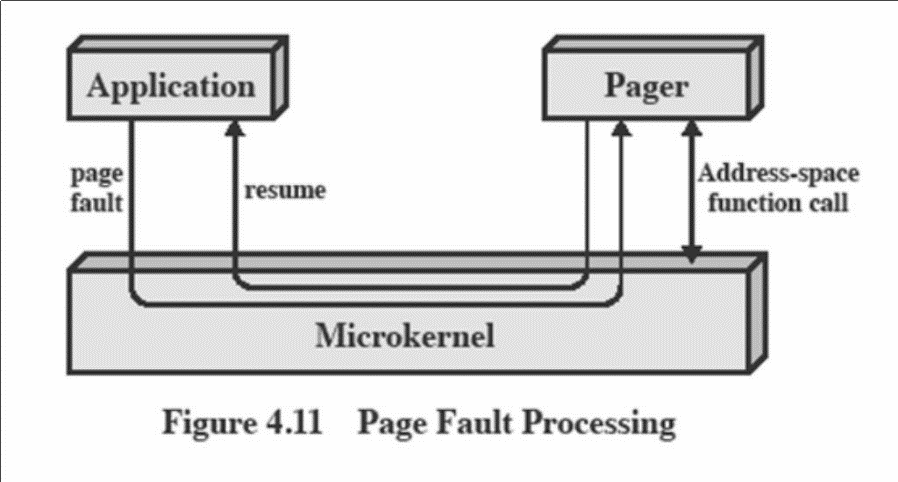
\includegraphics[width=4in]{img/pagefaultprocessing.png}
        \caption{Page Fault Processing}
    \label{fig:Page Fault Processing}
\end{figure}

a)	Primitief geheugenbeheer

De microkernel moet het hardware concept adresruimte ondersteunen om de implementatie van bescherming op procesniveau mogelijk te maken. Zolang de microkernel verantwoordelijk blijft voor het afbeelden van alle virtuele pagina’s op fysieke paginaframes, kan het grootste deel van het geheugenbeheer worden geïmplementeerd buiten de kernel.

Thread in toepassing verwijst naar een pagina niet in het hoofdgeheugen.

Paginafout en uitvoering valt terug op kernel.

Kernel stuurt bericht naar pagineerder met de aangeving naar welke pagina verwezen wordt.

Pagineerder kan besluiten de pagina te laden.

Is de pagina eenmaal beschikbaar, dan stuurt de pagineerder een hervattingbericht naar de toepassing.

b)	Communicatie tussen processen
De elementaire vorm van communicatie tussen processen of threads in een BS met een microkernel is het bericht. Een bericht bestaat uit:

\begin{itemize}
\item Een kop: info over verzendende en ontvangende proces.
\item Een romp: directe gegevens, verwijzing naar een blok gegevens en/of besturingsinformatie.
\end{itemize}

c)	I/O en interruptbeheer
Bij een microkernel architectuur is het mogelijk hardware-interrupts af te handelen als berichten en I/O poorten op te nemen in adresruimten. De microkernel kan interrupts herkennen maar handelt ze niet af. Is een interrupt ingeschakeld, dan is een bepaald proces op gebruikersniveau toegewezen aan de interrupt en onderhoudt de kernel de mapping.

Het omzetten van interrupts in berichten moet worden uitgevoerd door microkernel maar de microkernels is niet betrokken bij de interruptafhandeling voor specifieke apparaten.
